%% Copyright information
%% Copyright (c) 2023, Ignacio Slater M.
%% BSD Zero Clause License.

\subsubsection{Crossover}
\label{sec:bg:ga:var:cx}
  In genetic algorithms, a prominent variation operator is the 
  \emph{crossover}.
  This operator mirrors the genetic recombination seen in nature.\footnote{
    Also known as \emph{crossing-over} 
    in~\autocite{hollandAdaptationNaturalArtificial1992a}.
  }
  It facilitates the exchange of genetic material between two individuals, 
  spawning a new generation.

  \begin{definition}[Crossover operator]
  \label{def:crossover_operator}
    The crossover operator recombines genetic material from existing 
    individuals to create new ones.
    Formally, it is represented as:

    \[
      X :\: \mathbb{P} \times \mathbb{R} \times \cdots \to \mathbb{P};\;
      (P,\, \rho_X,\, \dots) \mapsto X(P,\, \rho_X,\, \dots)
    \]

    with the following parameters:

    \begin{itemize}
      \item \(\mathbb{P}\) -- the set of all possible populations,
      \item \(\mathbb{R}\) -- the set of real numbers,
      \item \(P\) -- the population under variation,
      \item \(\rho_X\) -- probability of applying the operator to an individual.
    \end{itemize}
  \end{definition}

  In our analysis, we employ a condensed version of the \emph{single-point 
  crossover} operator.\footnote{
    Refer to \vref{sec:keen:operators:crossover:single_point}.
  }
  This operator picks the first half of the genes from two parental figures and 
  births two new offspring by swapping these chosen genes. 

  Take, for instance, two parent individuals, \(I_1 = 1100\) and \(I_2 = 
  0001\).
  Utilizing the \textit{single-point crossover} operator, we select the first 
  half of the genes: 11 from \(I_1\) and 00 from \(I_2\).
  This exchange produces the offspring \(O_1 = 1101\) and \(O_2 = 0000\), 
  demonstrated in 
  \vref{fig:bg:ga:var:cx:single_point}.

  \begin{figure}[ht!]
    \centering
    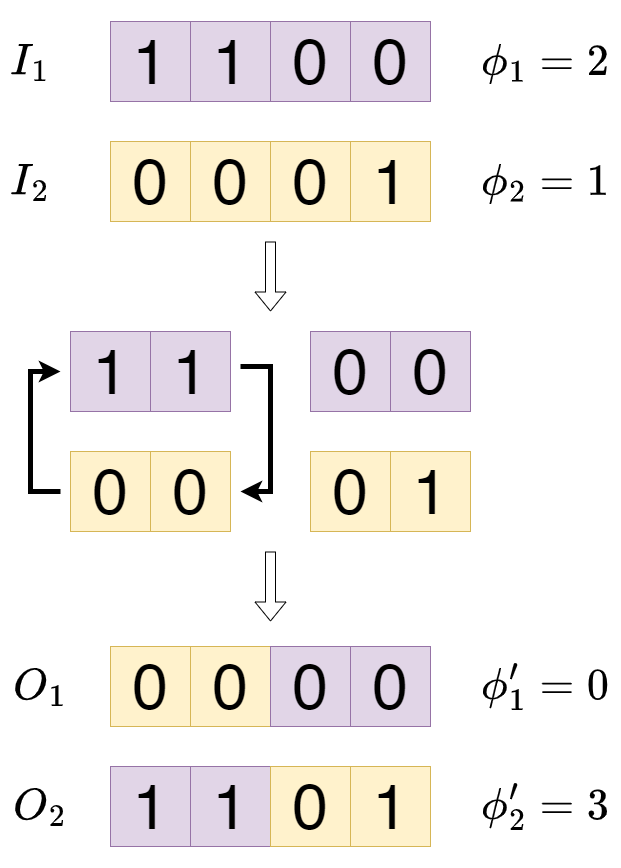
\includegraphics[width=0.3\textwidth]
      {img/theoretical_framework/Single-Point Crossover.png}
    \caption{Single-point crossover}
    \label{fig:bg:ga:var:cx:single_point}
  \end{figure}

  Following another iteration of the single-point crossover operator, we can 
  generate a result as shown in 
  \vref{tab:bg:ga:var:cx:single_point}, leading to a 
  new population \(\textbf{O} = \{(0000,\, 0),\, (1101,\, 3),\, (0101,\, 2)\}\).

  \begin{table}[ht!]
    \centering
    \begin{tabular}{|c|c|c|c|}
      \multicolumn{4}{c}{\textbf{Generation 0} \(\to\) \textbf{Generation 1}} \\
      \hline
      \hline
      \(\mathbf{I}\) & \(\Phi_\mathbf{I}\) & \(\mathbf{O}\) & \(\Phi_\mathbf{O}\) \\
      \hline
      \Gape[2pt][2pt]{\(\begin{bmatrix} 1100 \\ 0001 \end{bmatrix}\)}
      & \(\begin{bmatrix} 2 \\ 1 \end{bmatrix}\) 
      & \(\begin{bmatrix} 0000 \\ 1101 \end{bmatrix}\) 
      & \( \begin{bmatrix} 0 \\ 3 \end{bmatrix}\) \\
    \hline
    \(\begin{bmatrix} 0001 \\ 0100 \end{bmatrix}\) 
      & \Gape[2pt][2pt]{\(\begin{bmatrix} 1 \\ 1 \end{bmatrix}\)}
      & \(\begin{bmatrix} 0101 \\ \cdot \end{bmatrix}\)
      & \(\begin{bmatrix} 2 \\ \cdot \end{bmatrix}\) \\[0.5em]
      \hline
    \end{tabular}
    \caption{
      Illustration of the single-point crossover operation. 
      In this procedure, two parent individuals are selected and a cut point is 
      chosen. 
      Each offspring is then formed by combining the genes from the parents: 
      one gets the genes from the first part of the first parent and the second 
      part of the second parent, while the other gets the genes from the first 
      part of the second parent and the second part of the first parent. 
      Here, \(\cdot\) represents a \enquote{discarded} value (since according 
      to the survival rate, only three offspring need to be produced).
    }
    \label{tab:bg:ga:var:cx:single_point}
  \end{table}

  If we now use these offspring as-is to create the next generation, we would 
  obtain the population shown in 
  \vref{tab:bg:ga:var:cx:single_point:2}:

  \begin{table}[ht!]
    \centering
    \begin{tabular}{c | c | c }
      \multicolumn{3}{c}{\textbf{Generation 1}} \\
      \hline
      \hline
      \textbf{Individual} & \textbf{Binary String}  & \textbf{Fitness} \\
      \hline
      \(I_2\)             & \(0001\)                & 1 \\
      \(O_1\)             & \(0000\)                & 0 \\
      \(O_2\)             & \(1101\)                & 3 \\
      \(O_3\)             & \(0101\)                & 2
    \end{tabular}
    \caption{
      Population after applying the single-point crossover operator.
      Note that \(I_2\) is the survivor of the previous generation picked in 
      \vref{sec:bg:ga:select}.
    }
    \label{tab:bg:ga:var:cx:single_point:2}
  \end{table}

  \begin{table}[H]
    \centering
    \begin{tabular}{|c|c|c|}
      \hline
            & \textbf{Fitness} & \textbf{Individual}  \\
      \hline
      Best  & 3 & \(O_2\) \\
      Worst & 0 & \(O_1\) \\
      \hline
      \hline
      Average & \multicolumn{2}{c|}{1.25} \\
      \hline
      Standard deviation & \multicolumn{2}{c|}{1.291} \\
      \hline
    \end{tabular}
    \caption{
      Fitness of the population after applying the single-point crossover 
      operator.
      \enquote{Best} refers to the individual with the highest fitness, and 
      \enquote{Worst} refers to the individual with the lowest fitness
    }
    \label{tab:bg:ga:var:cx:single_point:fitness}
  \end{table}

  By the metrics in \vref{tab:bg:ga:var:cx:single_point:fitness}, the 
  population's average fitness rises from 1 to 1.25, with the fittest 
  individual's score jumping from 2 to 3.
  This uplift highlights the crossover operator's role in directing the search 
  towards enhanced solutions.

  While the crossover operation elevates the average population fitness, 
  incorporating a \emph{mutation} operator can further boost genetic 
  diversity\footnote{See \vref{def:diversity}.} and sidestep early convergence
  to inferior solutions.
  The subsequent section delves into this operation.
